\documentclass[11pt]{article}
\usepackage[margin=1in]{geometry}
\usepackage{amsmath,amssymb,amsthm,mathtools,bm}
\usepackage{booktabs,array,longtable}
\usepackage{enumitem}
\usepackage{xcolor}
\usepackage{tikz}
\usepackage{pgfplots}
\pgfplotsset{compat=1.17}
\usepackage[hidelinks]{hyperref}
\usepackage{microtype}

\setlist{itemsep=2pt,topsep=4pt}
\setlength{\parskip}{4pt}

\theoremstyle{plain}
\newtheorem{theorem}{Theorem}[section]
\newtheorem{proposition}[theorem]{Proposition}
\newtheorem{lemma}[theorem]{Lemma}
\newtheorem{corollary}[theorem]{Corollary}
\theoremstyle{definition}
\newtheorem{definition}[theorem]{Definition}
\newtheorem{assumption}[theorem]{Assumption}
\theoremstyle{remark}
\newtheorem{remark}[theorem]{Remark}
\newtheorem{example}[theorem]{Example}

\newcommand{\R}{\mathbb{R}}
\newcommand{\E}{\mathbb{E}}
\newcommand{\norm}[1]{\left\lVert #1 \right\rVert}
\newcommand{\abs}[1]{\left\lvert #1 \right\rvert}
\newcommand{\tr}{\mathsf{T}}
\newcommand{\sat}{\operatorname{sat}}
\newcommand{\softmin}{\operatorname{smin}}
\newcommand{\softplus}{\operatorname{sp}}
\DeclareMathOperator*{\argmin}{arg\,min}
\DeclareMathOperator*{\argmax}{arg\,max}
\DeclareMathOperator{\med}{med}

\newenvironment{takeaway}{\par\medskip\noindent\begin{minipage}{\linewidth}\hrule\smallskip\noindent\textbf{Takeaway.}~}{\par\smallskip\hrule\end{minipage}\par\medskip}

\title{\textbf{Ground Truth, Toronto 26}\\[4pt]\large Strategy and the math behind it: identifying ten hidden ODE systems\\ and forecasting 4,000 steps open loop}
\author{Dylan Ho}
\date{September 23, 2026}

\begin{document}
\maketitle

\begin{abstract}
\noindent This report turns the hackathon into a precise math problem and derives a strategy from it. Each simulator is a controlled ODE $\dot x = f(x,u;\theta,m)$ with hidden state, hidden parameters $\theta$ and a hidden choice $m$ of two out of three mechanisms. We get 2,000 noisy samples per system. We have to submit a function that, given a noisy initial observation and a 4,000-step control schedule, returns the whole trajectory without feedback. The main results: (1) fitting a grey-box ODE is mathematically sound, and contraction theory says exactly when a 4,000-step open-loop forecast stays accurate, and when it can't (integrators, limit cycles). (2) The metric $1/(1+|e|/\sigma)$ is a bounded, concave loss. It punishes steady bias much more than rare large misses. It turns "clip to physical bounds", "shrink oscillations toward their mean at long horizons" and "median ensembles" into provably good moves. (3) Fit on open-loop simulation error, never one-step prediction error: with noisy data, one-step fits are provably biased. (4) Design experiments to tell the three mechanism hypotheses apart, not just to fit parameters. Every tool comes with a statement of when it applies and what can go wrong.
\end{abstract}

\tableofcontents
\newpage

%=====================================================================
\section{Executive summary}
%=====================================================================

\paragraph{The game in one paragraph.} Ten simulators, each a hidden ODE. You pay one credit per tick and get 2,000 ticks per system. Resets are free, and a reset always puts the hidden state back to the same reference condition, set by the observed initial values. At scoring time, your \texttt{predict} gets a noisy starting observation and 4,000 future actions, and returns 4,000 predicted observations with no feedback. Per tick and observable you earn $1/(1+|e|/\sigma)$. The final score is the mean over all ticks, observables, 40 episodes and all ten systems. A missing system counts as zero.

\paragraph{The strategy.}
\begin{enumerate}
\item \textbf{Coverage first.} Every system is 10\% of the score, and persistence already beats a zero. Submit something valid for all ten on day one.
\item \textbf{Grey-box ODEs as the main model.} Write a structural ODE per family from its brief: compartments, queues, stocks, thermostat populations. Estimate its roughly 10--25 parameters by open-loop simulation error, and pick which two of the three mechanisms are on by held-out score. Few parameters plus the right structure is the only thing that extrapolates from 2,000 ticks to 4,000 (Section~\ref{sec:validity}).
\item \textbf{A black-box ladder as backup.} Persistence, then a multi-timescale Hammerstein lag, then a stable linear state space with input and output nonlinearities, then an ODE plus a residual correction. Each rung is stable by construction, and the best one per observable wins on validation (Section~\ref{sec:nonlinear}).
\item \textbf{Loss matched to the metric.} Train with a robust (Cauchy-type) loss on full rollouts. Clip every output to physical bounds. Shrink oscillations whose phase you can't hold over 4,000 ticks. Use medians to combine models (Section~\ref{sec:metric}).
\item \textbf{Experiments that look like the test.} Holds, pulse trains at 70--100\% of the pulse action with log-spread gaps, order-swapped pairs, single-then-joint controls. Plus the one discriminating experiment each brief suggests (Section~\ref{sec:design}).
\item \textbf{Zero-risk operations.} Spending is gated, logged and resumable, and every upload passes a local contract checker that mirrors the real sandbox. Upload finals explicitly between Sep 28 12:00 and Sep 30 12:00.
\end{enumerate}

%=====================================================================
\section{The problem, stated precisely}\label{sec:setup}
%=====================================================================

\subsection{The hidden system}
For one family, let $x(t)\in\R^n$ be the hidden state, $u(t)\in\mathcal U=\prod_{i=1}^{m}[\ell_i,h_i]$ the control and $y(t)\in\R^p$ the physical observables. The simulator is
\begin{equation}\label{eq:ode}
\dot x(t) = f\big(x(t),u(t);\theta,\mathsf m\big),\qquad y(t)=h\big(x(t),u(t);\theta\big),
\end{equation}
where $\theta\in\Theta\subset\R^d$ are the fixed physical parameters and $\mathsf m\subset\{A,B,C\}$ with $|\mathsf m|=2$ is the set of active mechanisms. Controls are held over each tick (\emph{zero-order hold}): $u(t)=u_k$ for $t\in[k,k+1)$. Writing $\Phi_\tau(x,u)$ for the flow of \eqref{eq:ode} over time $\tau$ with $u$ held constant, the exact sampled system is
\begin{equation}\label{eq:discrete}
x_{k+1}=F(x_k,u_k):=\Phi_1(x_k,u_k),\qquad y_{k+1}=h(x_{k+1},u_k),\qquad k=0,1,\dots
\end{equation}
So a continuous-time ODE sampled once per tick is \emph{exactly} a discrete-time nonlinear state-space model. Anything we say about \eqref{eq:discrete} holds for the simulator.

\subsection{What we observe}
A reset draws a true initial observation $y_0$ and sets the hidden state deterministically,
\begin{equation}\label{eq:reset}
x_0=\xi(y_0;\theta),
\end{equation}
where $\xi$ is the brief's fixed initialisation convention, e.g.\ ``waiting lists start empty'', ``warehouses half full'', or ``same asynchronous thermostat population at reference price 0.8''. We never see exact values. Every reading is noisy:
\begin{equation}
\tilde y_k = y_k + \varepsilon_k,\qquad \E\varepsilon_k=0,\quad \operatorname{Cov}\varepsilon_k=R\ \text{(unknown, possibly multiplicative)}.
\end{equation}

\subsection{What we must output}
Given $(\tilde y_0,\,u_{0:N-1})$ with $N=4000$, return $\hat y_{1:N}$. The score of one episode is
\begin{equation}\label{eq:score}
S=\frac{1}{Np}\sum_{k=1}^{N}\sum_{j=1}^{p} s\big(\hat y_{k,j}-y_{k,j};\sigma_j\big),\qquad s(e;\sigma)=\frac{1}{1+\abs{e}/\sigma},
\end{equation}
where $y$ is the \emph{noiseless} truth and $\sigma_j>0$ is a scale the organiser fixed from reference trajectories. There are 40 episodes per system, 10 in each of four categories (sustained, order, recovery, composition), and the overall score is the mean over the ten systems.

\subsection{What makes it hard}
\begin{itemize}
\item \textbf{Open loop and long.} Errors compound for 4,000 steps with no corrections.
\item \textbf{Extrapolation in time.} Budget $<$ horizon: we can never watch a full 4,000-tick trajectory.
\item \textbf{Structural uncertainty.} Even with perfect data we'd need to pick $\mathsf m$ out of 3 candidates.
\item \textbf{Partial observation.} $p\ll n$; many hidden states (fatigue, in-transit animals, layer temperatures) act only through their effects later on.
\end{itemize}

\subsection{What makes it easier}
\begin{itemize}
\item \textbf{Determinism and a known reset.} Given $y_0$, the full future is a deterministic function of the actions. There is no process noise and no random prehistory. Only measurement noise and our ignorance of $(\theta,\mathsf m)$ stand between us and a perfect forecast.
\item \textbf{The same world for everyone and every phase.} What we learn transfers to the final exactly.
\item \textbf{Known test structure.} The four schedule categories and the pulse rule (70--100\% of the way from recovery to pulse, per control) tell us which part of input space matters.
\end{itemize}

%=====================================================================
\section{What the metric rewards}\label{sec:metric}
%=====================================================================

Everything downstream (loss choice, clipping, how to handle oscillations, how to ensemble) follows from the shape of $s(e;\sigma)$.

\subsection{Basic properties}
Define the per-tick loss $\ell(e)=1-s(e;\sigma)=\dfrac{\abs e}{\sigma+\abs e}$.

\begin{proposition}\label{prop:loss}
$\ell$ is (i) bounded, $0\le\ell<1$; (ii) increasing in $\abs e$; (iii) concave in $\abs e$ on $[0,\infty)$; (iv) $\ell(e)=\abs e/\sigma - \abs e^2/\sigma^2+O(\abs e^3)$ near $0$.
\end{proposition}
\begin{proof}
With $r=\abs e\ge0$: $\ell=r/(\sigma+r)$, $\ell'=\sigma/(\sigma+r)^2>0$, $\ell''=-2\sigma/(\sigma+r)^3<0$. The expansion is the geometric series of $1/(1+r/\sigma)$.
\end{proof}

\begin{figure}[h]
\centering
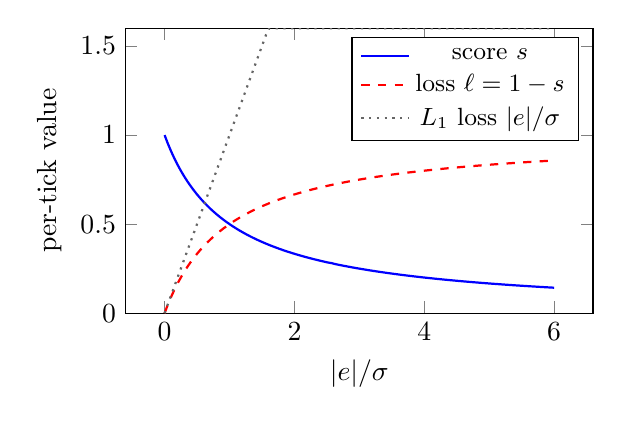
\begin{tikzpicture}
\begin{axis}[width=0.62\linewidth,height=5.2cm,xlabel={$|e|/\sigma$},ylabel={per-tick value},domain=0:6,samples=120,legend pos=north east,legend style={font=\small},ymin=0,ymax=1.6]
\addplot[thick,blue]{1/(1+x)}; \addlegendentry{score $s$}
\addplot[thick,red,dashed]{x/(1+x)}; \addlegendentry{loss $\ell=1-s$}
\addplot[thick,black!60,dotted]{min(x,1.6)}; \addlegendentry{$L_1$ loss $|e|/\sigma$}
\end{axis}
\end{tikzpicture}
\caption{The score is steep near zero and flat far away. Small errors cost almost linearly, and huge errors cost at most 1.}
\end{figure}

What this means in practice:
\begin{itemize}
\item \textbf{Divergence is capped, bias is not.} A forecast that blows up on 5\% of ticks loses at most 0.05. A steady bias of $0.5\sigma$ on \emph{every} tick loses $1/3$. Over 4,000 ticks, getting the steady state right matters much more than getting the transients perfect.
\item \textbf{Near zero it behaves like $L_1$.} Once you are within about $\sigma$, the metric acts like mean absolute error, so median-type predictions are right (Section~\ref{sec:pointforecast}).
\item \textbf{The organiser's $\sigma$ is unknown, but rankings mostly aren't sensitive to it.} If model $A$ has $\abs{e^A_{k,j}}\le\abs{e^B_{k,j}}$ at every tick, $A$ scores at least as well for \emph{any} $\sigma$. When that doesn't hold, we rank using the average score over $\sigma\in\{0.5,1,2\}\times\hat\sigma$, where $\hat\sigma_j$ is the standard deviation of observable $j$ across our data.
\end{itemize}

\subsection{Clipping to physical bounds never hurts}
\begin{lemma}[Projection]\label{lem:proj}
Let the true value satisfy $y\in[a,b]$ (with $a=-\infty$ or $b=+\infty$ allowed) and let $\Pi(z)=\min(\max(z,a),b)$. Then $\abs{\Pi(z)-y}\le\abs{z-y}$ for every $z$. Hence $s(\Pi(z)-y)\ge s(z-y)$.
\end{lemma}
\begin{proof}
If $z\in[a,b]$ then $\Pi(z)=z$. If $z>b\ge y$ then $\abs{\Pi(z)-y}=b-y< z-y$. The case $z<a$ is symmetric. The score is decreasing in $\abs e$.
\end{proof}
So every output is clipped to its known physical range: nonnegativity for counts, levels and flows, $[0,1]$ for shares and quality indices, and $\text{spend}\le\text{budget\_cap}$ for the ad auction. The same lemma holds for a soft plausibility box built from the data, \emph{as long as} the truth really stays inside it. That's why the soft box gets a 20\% margin.

\subsection{Optimal point forecast when we are unsure}\label{sec:pointforecast}
Suppose that at some tick our belief about the truth is a distribution $P$ of a random $Y$. The best point forecast is
\begin{equation}
a^\star=\argmin_a \E_P\,\ell(Y-a)=\argmax_a\E_P\frac{\sigma}{\sigma+\abs{Y-a}}.
\end{equation}
\begin{itemize}
\item If $P$ is concentrated on a scale $\ll\sigma$, then by Prop.~\ref{prop:loss}(iv) $\ell\approx\abs{\cdot}/\sigma$, and $a^\star\approx\med(Y)$.
\item If $P$ is spread on a scale $\gg\sigma$, $\ell$ is concave and nearly flat, and $a^\star$ moves toward a \emph{mode} (the place with the most probability within $\pm\sigma$).
\end{itemize}
In both cases the mean is \emph{not} the target. That matters for ensembles and for oscillations.

\subsection{Median ensembles are robust}
\begin{proposition}\label{prop:median}
Let $M$ models give forecasts $z_1,\dots,z_M$ at some tick, and suppose more than $M/2$ of them lie in $[y-\delta,y+\delta]$. Then $\abs{\med(z)-y}\le\delta$.
\end{proposition}
\begin{proof}
Sort the $z$'s. The median has at least $\lceil M/2\rceil$ values on each side. If it were above $y+\delta$, then at least $\lceil M/2\rceil$ values would be above $y+\delta$, leaving fewer than $M/2$ inside the interval, a contradiction. The same argument works below.
\end{proof}
A mean ensemble can be pulled arbitrarily far by one diverging member. The median ignores a minority of bad members completely, which is exactly the failure mode (occasional divergence) we fear.

\subsection{Oscillations and the ``shrink to the mean'' result}\label{sec:osc}
Some systems oscillate (predator--prey cycles, thermostatic load rebounds). Suppose the truth is $y_k=\mu+A\sin(\omega k+\phi)$, and our model has the right $\mu,A$ but a slightly wrong frequency $\hat\omega=\omega+\Delta\omega$. The phase error $\Delta\omega\,k$ grows linearly, so after roughly $\pi/\abs{\Delta\omega}$ ticks the forecast is in \emph{anti-phase}.

\begin{proposition}[Wrong-phase oscillation vs.\ the mean]\label{prop:phase}
Let $\varphi\sim\mathrm U[0,2\pi)$ be the true phase and $\delta$ the phase error, with $\delta$ independent of $\varphi$ and uniform (fully decorrelated). Then
\[
\E\abs{y-\mu}=\tfrac{2}{\pi}A\approx0.64A,\qquad \E\abs{y-\hat y_{\text{osc}}}=\tfrac{8}{\pi^2}A\approx0.81A.
\]
So once the phase is lost, predicting the mean $\mu$ has about 21\% less absolute error than predicting a confident wrong-phase oscillation.
\end{proposition}
\begin{proof}
$\E\abs{\sin\varphi}=2/\pi$. For the oscillator forecast, $\sin\varphi-\sin(\varphi+\delta)=-2\cos(\varphi+\delta/2)\sin(\delta/2)$, so $\E\abs{\cdot}=2\cdot\frac{2}{\pi}\cdot\E\abs{\sin(\delta/2)}=\frac4\pi\cdot\frac2\pi A$.
\end{proof}

A smoother version of the same idea: if the phase error diffuses, $\delta_k\sim\mathcal N(0,\kappa k)$, then the conditional mean of the truth is
\begin{equation}\label{eq:shrink}
\E[y_k]=\mu+A\,e^{-\kappa k/2}\sin(\hat\omega k+\phi),
\end{equation}
because $\E\cos\delta=e^{-\operatorname{Var}\delta/2}$ for Gaussian $\delta$. So the best forecast \textbf{damps the predicted oscillation at a rate set by how uncertain the phase is}. In practice we estimate $\kappa$ by validation, e.g.\ by fitting the shrink rate that maximises the validation score. This isn't a hack. It's the right answer when the phase really is uncertain.

\begin{figure}[h]
\centering
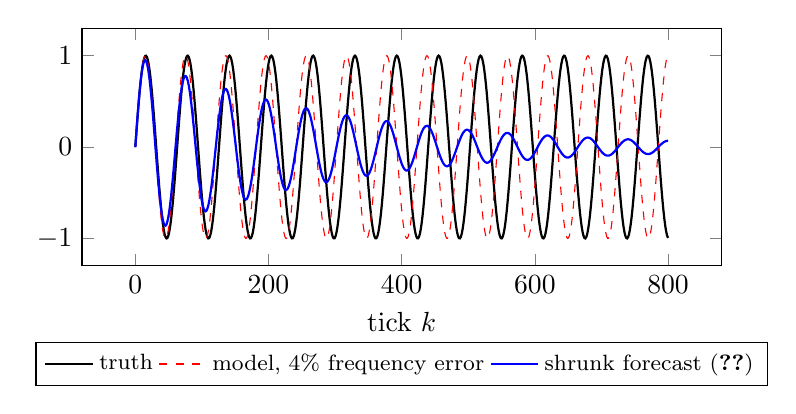
\begin{tikzpicture}
\begin{axis}[width=0.8\linewidth,height=4.6cm,xlabel={tick $k$},domain=0:800,samples=600,legend style={font=\footnotesize,at={(0.5,-0.32)},anchor=north},legend columns=3,ymin=-1.3,ymax=1.3]
\addplot[black,thick]{sin(deg(0.1*x))}; \addlegendentry{truth}
\addplot[red,dashed]{sin(deg(0.104*x))}; \addlegendentry{model, 4\% frequency error}
\addplot[blue,thick]{exp(-x/300)*sin(deg(0.104*x))}; \addlegendentry{shrunk forecast \eqref{eq:shrink}}
\end{axis}
\end{tikzpicture}
\caption{With a 4\% frequency error the forecast is a quarter-cycle off by tick $\approx400$ and in anti-phase by tick $\approx800$. The shrunk forecast gives up amplitude as it loses confidence in the phase.}
\end{figure}

\subsection{Training loss}
We want to maximise \eqref{eq:score}, but $\ell$ is not differentiable at 0 and it is non-convex. Standard trust-region least squares (SciPy \texttt{least\_squares}) handles robust losses of the form $\rho(r^2)$. We use the Cauchy loss
\begin{equation}
\rho_{\text{C}}(r)=\log\!\big(1+(r/c)^2\big),\qquad r=\frac{\hat y-\tilde y}{\hat\sigma},
\end{equation}
with $c\approx1$. Like $\ell$, it is quadratic-then-flat: the influence $\psi(r)=\rho'(r)$ goes to zero as $\abs r\to\infty$, so a few ticks where the model is far off (a transient in the wrong place) don't dominate the fit. MSE, by contrast, would bend the whole model to cut the largest errors, which the metric barely rewards. We also check every candidate with the \emph{exact} metric on held-out runs. The surrogate only has to point the optimiser in the right direction.

\begin{takeaway}
Get the steady states right, clip to physics, damp oscillations you can't phase-lock, combine models with medians, and train with a bounded-influence loss.
\end{takeaway}

%=====================================================================
\section{Is fitting an ODE a valid strategy? The math}\label{sec:validity}
%=====================================================================

We now check the core bet carefully: we write a parametric ODE $\dot x=\hat f(x,u;\hat\theta,\hat{\mathsf m})$, fit it to data, and integrate it for 4,000 ticks. Four questions need answers:
\begin{enumerate}[label=(Q\arabic*)]
\item Is the model well defined, i.e.\ does it have a unique, bounded solution for every allowed schedule?
\item If the parameters are slightly wrong, how wrong is the forecast after 4,000 ticks?
\item Does the numerical integrator reproduce the ODE faithfully?
\item Can the parameters and the mechanism set actually be learned from 2,000 noisy ticks?
\end{enumerate}

\subsection{(Q1) Existence, uniqueness, positivity and boundedness}
\begin{theorem}[Picard--Lindelöf, piecewise-constant input]\label{thm:pl}
Suppose that for each fixed $u\in\mathcal U$, $x\mapsto f(x,u)$ is Lipschitz on a set $K$ with constant $L_x$, and $K$ is forward invariant (solutions starting in $K$ stay in $K$). Then for every piecewise-constant schedule and every $x_0\in K$ there is a unique solution on $[0,\infty)$, and it stays in $K$.
\end{theorem}
\begin{proof}[Sketch]
On each tick the input is constant, so the standard theorem gives a unique solution on $[k,k+1]$. Forward invariance prevents escape, so the solution continues. Concatenating the ticks gives the global solution.
\end{proof}
How we make sure the hypotheses hold in our models:
\begin{itemize}
\item \textbf{Lipschitz nonlinearities only.} Mass-action terms ($\beta SI$), Michaelis--Menten and Holling type II ($\frac{aX}{1+bX}$), softplus, $\tanh$, and even $\min$/$\max$ are all Lipschitz on bounded sets. We avoid $\sqrt{x}$ at $0$ and $1/x$ terms.
\item \textbf{Positivity (quasi-positivity).} If $f_i(x,u)\ge0$ whenever $x_i=0$ and $x\ge0$, then the nonnegative orthant is forward invariant. Compartment and queue models satisfy this when every outflow of state $i$ is proportional to $x_i$ or capped by it. We write every outflow as $x_i\cdot(\text{rate})$ or $\min(\text{demand},\,x_i/\tau)$.
\item \textbf{Boundedness (dissipativity).} If there is a function $V(x)=c^\tr x$ (for example, total population or total volume) with $\dot V\le \alpha-\beta V$, then $V(t)\le\max\{V(0),\alpha/\beta\}$ for all $t$. Every family has a natural candidate (people, vehicles, water, goods, animals) with finite inflow and outflow proportional to stock. Where the physics doesn't guarantee a bound, we add a capacity (logistic term or buffer size) and also clip in the integrator.
\end{itemize}

\subsection{(Q2) How parameter error propagates over 4,000 ticks}
This is the central question. Let $x(t)$ be the true trajectory and $\hat x(t)$ the model's, with the same inputs. Write $d(x,u)=\hat f(x,u)-f(x,u)$ for the model error in the vector field.

\paragraph{The pessimistic bound.} Grönwall's inequality gives
\begin{equation}\label{eq:gronwall}
\norm{\hat x(t)-x(t)}\le e^{L_xt}\norm{\hat x_0-x_0}+\frac{\bar d}{L_x}\left(e^{L_xt}-1\right),\qquad \bar d=\sup\norm{d}.
\end{equation}
With $t=4000$, this is useless: it allows exponential error growth. If the true systems behaved like this, no method could forecast them.

\paragraph{The useful bound: contraction.}
\begin{definition}[Contraction, Lohmiller--Slotine]
The system $\dot x=f(x,u)$ is \emph{contracting} on $K$ at rate $\lambda>0$ in a constant metric $M\succ0$ if, for all $x\in K$ and $u\in\mathcal U$,
\[
\frac{\partial f}{\partial x}^{\!\tr}M+M\frac{\partial f}{\partial x}\preceq-2\lambda M.
\]
\end{definition}
\begin{theorem}[Forecast error under contraction]\label{thm:contraction}
Let $K$ be convex and forward invariant. If the \emph{model} $\hat f$ is contracting on $K$ at rate $\lambda$ in metric $M$ (norm $\norm{v}_M=\sqrt{v^\tr Mv}$), then for any input schedule
\[
\norm{\hat x(t)-x(t)}_M\le e^{-\lambda t}\norm{\hat x_0-x_0}_M+\frac{\bar d_M}{\lambda}\left(1-e^{-\lambda t}\right)\le e^{-\lambda t}\norm{\hat x_0-x_0}_M+\frac{\bar d_M}{\lambda},
\]
where $\bar d_M=\sup_{x\in K,u}\norm{\hat f(x,u)-f(x,u)}_M$ is the size of the vector-field mismatch along the truth.
\end{theorem}
\begin{proof}
Treat the truth as a perturbed solution of the model: $\dot x=\hat f(x,u)-d(x,u)$. Let $e=\hat x-x$. Then $\dot e=\hat f(\hat x,u)-\hat f(x,u)+d(x,u)$. By the mean-value theorem in integral form, $\hat f(\hat x)-\hat f(x)=J e$ with $J=\int_0^1\partial_x\hat f(x+se)\,ds$, and contraction gives $e^\tr M J e\le-\lambda\norm{e}_M^2$. Hence
$\tfrac{d}{dt}\tfrac12\norm{e}_M^2\le-\lambda\norm{e}_M^2+\norm{e}_M\norm{d}_M$, i.e.\ $\tfrac{d}{dt}\norm{e}_M\le-\lambda\norm{e}_M+\bar d_M$. Comparison with the linear ODE $\dot v=-\lambda v+\bar d_M$ gives the result.
\end{proof}

\noindent Read it this way:
\begin{itemize}
\item \textbf{Initial-state errors are forgotten} at rate $\lambda$. A noisy $\tilde y_0$ only hurts the first $\sim\!3/\lambda$ ticks.
\item \textbf{Parameter errors produce a bounded, horizon-independent error} of size $\bar d_M/\lambda$. A forecast that's good at tick 500 is equally good at tick 4,000. This is why a model fitted on 2,000 ticks can be trusted at 4,000.
\item \textbf{Well-damped systems are forgiving; slow modes are not.} $\lambda$ is set by the slowest decay rate. A fatigue or wear state with a 1,000-tick time constant has $\lambda\approx10^{-3}$ and amplifies vector-field errors by $10^3$. Slow states are where the budget should go (Section~\ref{sec:design}).
\end{itemize}

Most of our families are contracting in practice: queues drain, epidemics burn out or settle, reservoirs spill and release, inventories get pulled by orders. The dangerous cases are exactly those that aren't:

\paragraph{Case 1: integrators ($\lambda=0$).} A stock with $\dot L=q_{\text{in}}-q_{\text{out}}$ and no restoring force (reservoir level, inventory with no feedback) accumulates rate errors linearly:
\begin{equation}
\abs{\hat L(t)-L(t)}\le\abs{\hat L_0-L_0}+t\,\sup\abs{\Delta q}.
\end{equation}
A rate error of $0.1\%$ of flow grows to $4$ flow-units' worth of level after 4,000 ticks. The fixes are structural: (a) get the mass balance exactly right; for the reservoir, level is literally the running sum of inflow minus outflow, and both are observed, so the balance can be checked on data; (b) model the saturations that end up bounding the stock (spillway, empty-tank cutoff, warehouse capacity), which restores contraction once the stock hits them.

\paragraph{Case 2: limit cycles.} A Lotka--Volterra-type cycle is neutrally stable \emph{along} the orbit: amplitude errors decay but phase errors don't. Phase drifts linearly with any period error, and Prop.~\ref{prop:phase} and \eqref{eq:shrink} apply: at long horizons, damp toward the cycle mean.

\paragraph{Case 3: multistability.} If the system has several equilibria (e.g.\ congestion vs.\ free flow, epidemic vs.\ extinction), a small error can put the forecast in the wrong basin, and the error then stays $O(1)$ forever. That calls for dedicated experiments near the boundary (traffic spillback, supply-chain rework loops) and, when in doubt, the median ensemble.

\subsection{(Q3) Integrating the ODE: RK4, step size and stiffness}
Inside \texttt{predict} we integrate the model with classical 4th-order Runge--Kutta and $n_{\text{sub}}$ sub-steps per tick, $h=1/n_{\text{sub}}$.
\begin{itemize}
\item \textbf{Accuracy.} Local error is $O(h^5)$ and global error over a fixed interval is $O(h^4)$. For contracting systems the global error doesn't grow with the horizon (Theorem~\ref{thm:contraction} applied to the numerical scheme as a perturbation).
\item \textbf{Stability.} For linearised dynamics with eigenvalues $\mu_i$, RK4 is stable iff $h\mu_i$ lies in its stability region, which on the negative real axis extends to $h\abs{\mu}\lesssim2.78$. Fast modes with time constants $\tau<0.36h$ therefore blow up numerically. Rule: $n_{\text{sub}}\ge\lceil 1/(2.5\,\tau_{\min})\rceil$.
\item \textbf{It doesn't need to match the simulator's integrator.} The organisers' integrator is unknown. We fit $\theta$ \emph{through} our integrator, so any fixed discretisation error is absorbed into $\hat\theta$. What matters is that the \emph{discrete} map we fit matches the discrete data.
\item \textbf{Cost.} With $n_{\text{sub}}=4$, a rollout is $16\times4000=64{,}000$ evaluations of $f$. At $\sim\!15\,\mu$s each that is $\sim\!1$\,s per episode, so 40 episodes take $\sim\!40$\,s. The sandbox allows 1,200\,s.
\end{itemize}

\subsection{Non-smooth parts: saturations, buffers and switching}
Briefs mention finite buffers, ``orders withdraw only available stock'' and thermostats that switch at thresholds. These make $f$ Lipschitz but not differentiable (e.g.\ $\min(a,b)$). That's fine for existence (Theorem~\ref{thm:pl}). The problem is fitting: gradients jump. We replace hard kinks with smooth versions whose error is bounded:
\begin{lemma}[Smooth minimum]
For $\kappa>0$, $\softmin_\kappa(a,b)=-\kappa^{-1}\log\!\big(e^{-\kappa a}+e^{-\kappa b}\big)$ satisfies $\min(a,b)-\tfrac{\log2}{\kappa}\le\softmin_\kappa(a,b)\le\min(a,b)$.
\end{lemma}
\begin{proof}
With $a\le b$: $e^{-\kappa a}\le e^{-\kappa a}+e^{-\kappa b}\le2e^{-\kappa a}$. Take $-\kappa^{-1}\log$.
\end{proof}
Similarly $\softplus_\kappa(z)=\kappa^{-1}\log(1+e^{\kappa z})$ approximates $\max(z,0)$ within $\log2/\kappa$. We make $\kappa$ a fitted parameter, or fix it at about $10/(\text{typical scale})$. Thresholds become sigmoids with fitted steepness.

\subsection{Delays: turning DDEs into ODEs}
Briefs talk about pipelines: orders ``move through preparation and execution'', conveyors ``retain their travel commitment'', animals ``in transit''. A pure delay $\dot x(t)=g(x(t-\tau))$ makes the model a delay differential equation, which has an infinite-dimensional state. The \emph{linear chain trick} replaces it with $k$ first-order stages:
\begin{equation}\label{eq:chain}
\dot z_1=\tfrac{k}{\tau}(v-z_1),\quad \dot z_i=\tfrac{k}{\tau}(z_{i-1}-z_i),\ i=2..k,\qquad \text{output } z_k.
\end{equation}
\begin{proposition}
The impulse response of \eqref{eq:chain} is the Erlang density with mean $\tau$ and variance $\tau^2/k$. As $k\to\infty$ it converges to the pure delay $\delta(t-\tau)$.
\end{proposition}
So a pipeline is modelled as a chain of 3--8 stages. This is also realistic: physical pipelines disperse (not every order takes exactly $\tau$), and $k$ becomes a parameter that sets how much the delay smears.

\subsection{(Q4) Can the parameters be learned?}
\paragraph{Structural identifiability.} Two parameter vectors are indistinguishable if they produce the same output for \emph{every} input schedule. Examples: in $\dot x=-a x+bu,\ y=cx$, only $a$ and $bc$ are identifiable, not $b$ and $c$ separately. This is harmless for forecasting, since indistinguishable parameters give identical forecasts. The practical rule is to \emph{fix or tie} such combinations (e.g.\ set $c=1$) so the optimiser doesn't wander.

\paragraph{Practical identifiability (Fisher information).} With Gaussian noise, the Fisher information about $\theta$ from a run with actions $u$ is
\begin{equation}\label{eq:fisher}
\mathcal I(\theta;u)=\sum_{k}S_k^\tr R^{-1}S_k,\qquad S_k=\frac{\partial y_k}{\partial\theta},
\end{equation}
where $S_k$ follows the \emph{sensitivity equations}, obtained by differentiating \eqref{eq:ode}:
\begin{equation}
\frac{d}{dt}\frac{\partial x}{\partial\theta}=\frac{\partial f}{\partial x}\frac{\partial x}{\partial\theta}+\frac{\partial f}{\partial\theta},\qquad \frac{\partial x}{\partial\theta}(0)=\frac{\partial\xi}{\partial\theta}.
\end{equation}
By Cramér--Rao, any unbiased estimate has $\operatorname{Cov}(\hat\theta)\succeq\mathcal I^{-1}$. Small eigenvalues of $\mathcal I$ mark ``sloppy'' directions that the data don't pin down. Two consequences:
\begin{itemize}
\item \textbf{Only the sloppiness that matters for the test counts.} What we need is the forecast variance on test schedules, $\operatorname{Var}(\hat y^{\text{test}})\approx G\,\mathcal I^{-1}G^\tr$ with $G=\partial y^{\text{test}}/\partial\theta$. If the test schedules are like the training schedules, sloppy directions barely move the forecast. That's why experiments should look like the test.
\item \textbf{Inputs create information.} Parameters of a mechanism that's never excited have zero sensitivity and can't be learned. Experiments must excite each mechanism (Section~\ref{sec:design}).
\end{itemize}

\paragraph{The initial state is free information.} Because $x_0=\xi(y_0;\theta)$ is a fixed function (no random hidden prehistory), the initial transient is \emph{repeatable}. That's what makes 40 short runs from reset nearly as informative as one long run, and it's why reset transients deserve careful fitting: they appear in all 40 scored episodes.

\begin{takeaway}
Fitting an ODE is valid when (a) the model is well posed (Lipschitz, positive, bounded), which we guarantee by construction; (b) the dynamics contract, so the forecast error stays bounded at $\bar d/\lambda$ over 4,000 ticks; (c) the step size respects the fastest mode; and (d) the experiments excite every parameter the test depends on. Where contraction fails (integrators, cycles, multiple equilibria), we know in advance and treat those cases specially.
\end{takeaway}

%=====================================================================
\section{Estimation: how the parameters are fitted}\label{sec:estimation}
%=====================================================================

\subsection{Output error, not equation error}
There are two ways to fit a dynamical model.
\begin{itemize}
\item \textbf{Equation error (one-step prediction):} regress $\tilde y_{k+1}$ on $(\tilde y_k,u_k)$. It's fast and convex for linear-in-parameter models.
\item \textbf{Output error (simulation error):} simulate the model from the initial condition through all actions and compare its trajectory with the data: $\min_\theta\sum_k\rho\big(\hat y_k(\theta)-\tilde y_k\big)$.
\end{itemize}
The scorer runs our model in open loop, which is exactly output error. Equation error is also \emph{biased} when observations are noisy:

\begin{proposition}[Errors-in-variables attenuation]\label{prop:eiv}
Let $y_{k+1}=a\,y_k+b\,u_k$ with $\abs a<1$, observed as $\tilde y_k=y_k+\varepsilon_k$ with white noise of variance $r$ and $u$ white with variance $q$, independent of $\varepsilon$. The one-step least-squares estimate of $a$ converges to
\[
\hat a\;\to\;a\,\frac{\operatorname{Var}(y)}{\operatorname{Var}(y)+r}\;<\;a\quad(a>0).
\]
\end{proposition}
\begin{proof}
$\hat a\to\operatorname{Cov}(\tilde y_{k+1},\tilde y_k)/\operatorname{Var}(\tilde y_k)$ (the $u$ regressor is uncorrelated with $\tilde y_k$ in steady state, so it doesn't change the limit). The numerator is $\operatorname{Cov}(y_{k+1},y_k)=a\operatorname{Var}(y)$ because the noises are independent. The denominator is $\operatorname{Var}(y)+r$.
\end{proof}
A smaller $\hat a$ means a shorter time constant: $\tau=-1/\ln a$. With $a=0.99$ ($\tau\approx100$) and a 5\% noise-to-signal variance ratio, $\hat a\approx0.943$, so $\hat\tau\approx17$. The model forgets six times too fast, and over 4,000 ticks it misses every slow effect. \textbf{So we use one-step fits only as initial guesses and always finish with output error.}

\subsection{The optimisation problem}
With runs $r=1..R$, each with initial reading $\tilde y_0^{(r)}$, actions $u^{(r)}$ and readings $\tilde y^{(r)}$:
\begin{equation}\label{eq:oe}
\hat\theta_{\mathsf m}=\argmin_{\theta\in\Theta}\ \sum_{r=1}^{R}\frac{1}{T_r}\sum_{k=1}^{T_r}\sum_{j=1}^{p}\rho_C\!\left(\frac{\hat y^{(r)}_{k,j}(\theta,\mathsf m)-\tilde y^{(r)}_{k,j}}{\hat\sigma_j}\right)+\gamma\norm{\vartheta-\vartheta_{\text{prior}}}^2.
\end{equation}
Implementation details:
\begin{itemize}
\item \textbf{Reparametrisation.} Rates, capacities and time constants are positive and span orders of magnitude, so we optimise $\vartheta=\log\theta$ inside wide bounds. This also makes the problem better conditioned.
\item \textbf{Weighting.} Each run is weighted by $1/T_r$ so one long run doesn't drown out many short reset runs. Each observable is divided by $\hat\sigma_j$ so the fit matches the metric's scaling.
\item \textbf{Solver.} Trust-region reflective least squares with the Cauchy loss. The Jacobian comes from finite differences or the sensitivity equations.
\item \textbf{Non-convexity.} Output-error landscapes for nonlinear ODEs have many local minima, especially with oscillations. We use (a) multi-start from 8 Latin-hypercube points; (b) a curriculum: fit short horizons first (first 100 ticks of each run), then the full runs; (c) \emph{multiple shooting} for long runs: split into segments with free initial states $s_i$, and add the continuity penalty $\sum_i\norm{\Phi(s_i)-s_{i+1}}^2$, which is tightened toward equality. Multiple shooting provably smooths the landscape because each segment is short enough to avoid the exponential sensitivity of long integrations.
\item \textbf{Weak prior $\gamma$.} Keeps parameters that the data can't identify near sensible values, instead of letting them drift to extreme bounds.
\end{itemize}

\subsection{Picking the two active mechanisms}
Exactly two of the three candidate mechanisms are on, so there are three structural hypotheses, $\mathsf m\in\{AB,AC,BC\}$. Fit each with \eqref{eq:oe} and score each on held-out runs with the exact metric. With nested models (switching a mechanism off amounts to setting its gain to zero), the fit with all three on can never be worse in-sample. That's why selection has to be out-of-sample, or at least penalised: $\text{BIC}=2\,\text{NLL}+d\log N$ penalises the extra parameters. We report both and use held-out score as the decision rule.

A useful trick: fit the \emph{ABC} model (all three on) first. If one mechanism's fitted strength is statistically zero (its confidence interval from $\mathcal I^{-1}$ covers 0), that's direct evidence it's the inactive one.

\subsection{Denoising the initial observation}
At test time we only get $\tilde y_0=y_0+\varepsilon_0$. Because $x_0=\xi(y_0)$, an error in $y_0$ leaks into the hidden state. The best linear estimate of $y_0$, assuming across-episode variance $\Sigma_0$ around a mean $\mu_0$ and noise covariance $R$, is the Kalman/James--Stein shrink
\begin{equation}\label{eq:shrink0}
\hat y_0=\mu_0+\Sigma_0(\Sigma_0+R)^{-1}(\tilde y_0-\mu_0).
\end{equation}
Both ingredients are \emph{free}: resets cost nothing, so dozens of reset readings give $\operatorname{Cov}(\tilde y_0)=\Sigma_0+R$, and $R$ comes from the scatter of readings during long holds where the truth is flat. When $R\ll\Sigma_0$ the shrink does nothing, but it never hurts in expectation. Better still, the model can learn the initial map directly, since it's fitted on runs that start from $\tilde y_0$.

%=====================================================================
\section{Modelling the nonlinear parts: a toolkit}\label{sec:nonlinear}
%=====================================================================

The grey-box ODE is the main bet, but if the structure we guess is wrong, a flexible model is a safer fallback. Every tool below is chosen to be \emph{stable by construction}, because divergence over 4,000 ticks is the biggest risk (Section~\ref{sec:metric}).

\subsection{Block-oriented models (Hammerstein, Wiener)}
Many physical systems are ``static nonlinearity + linear dynamics''.
\begin{itemize}
\item \textbf{Hammerstein:} $u\to\phi(u)\to$ linear dynamics $\to y$. Right when the controls have diminishing returns (e.g.\ mask effectiveness) but the internal dynamics are linear.
\item \textbf{Wiener:} $u\to$ linear dynamics $\to g(\cdot)\to y$. Right when the output saturates (shares in $[0,1]$, speeds capped by free flow).
\item \textbf{Hammerstein--Wiener:} both. We choose $g^{-1}$ from the observable's range: $\operatorname{logit}$ for $[0,1]$ quantities, $\log(1+y/s)$ for positive quantities spanning orders of magnitude, affine otherwise. Modelling in transformed space automatically keeps outputs in range.
\end{itemize}

\paragraph{L1: multi-timescale lag.} For each observable, $K=3$ first-order filters driven by input features:
\begin{equation}
z^{(i)}_{k+1}=a_i z^{(i)}_k+(1-a_i)W_i\phi(u_k),\qquad \hat y_k=g\Big(c+\sum_i z^{(i)}_k\Big),\qquad a_i=\sigma(\eta_i)\in(0,1).
\end{equation}
Its steady state for a held input is $y^\star(u)=g\big(c+\sum_iW_i\phi(u)\big)$, a learned \emph{equilibrium map}. Its time constants are $\tau_i=-1/\ln a_i$, initialised at about $2$, $20$ and $200$ ticks. It is stable for every parameter value since $\abs{a_i}<1$. It captures sustained operation (the steady state) and first-order recovery well. It cannot represent overshoot or rebound; that's L2's job.

\subsection{Stable linear state space with complex poles (L2)}
\begin{equation}
x_{k+1}=Ax_k+B\phi(u_k),\qquad \hat y_k=g(Cx_k+D\phi(u_k)+c).
\end{equation}
The only real risk is $A$ having an eigenvalue outside the unit circle. We make that impossible with a \emph{modal parametrisation}: $A=\operatorname{blkdiag}(A_1,\dots)$ with $2\times2$ blocks
\begin{equation}
A_i=r_i\begin{pmatrix}\cos\vartheta_i&-\sin\vartheta_i\\ \sin\vartheta_i&\cos\vartheta_i\end{pmatrix},\qquad r_i=r_{\max}\,\sigma(\rho_i)<1,
\end{equation}
whose eigenvalues are $r_ie^{\pm i\vartheta_i}$. Complex poles give \emph{damped oscillation}, which is exactly the rebound after a thermostat price pulse or a predator--prey swing. Real $1\times1$ blocks give plain decay. Any real diagonalisable $A$ is similar to this form, so no generality is lost. Initialise with subspace identification (N4SID: SVD of a block-Hankel matrix of input--output data), which gives a consistent linear estimate in one shot. Then refine with output error.

\paragraph{Why linear state space can model nonlinear systems (Koopman view).} For a nonlinear map $x_{k+1}=F(x_k)$, the Koopman operator $\mathcal K\psi=\psi\circ F$ acts \emph{linearly} on functions $\psi$ of the state. If a finite set of ``observables'' $\psi_1..\psi_n$ spans an (approximately) invariant subspace, the lifted state $z=\psi(x)$ evolves linearly, $z_{k+1}\approx Az_k$. L2 learns such a lifted representation implicitly. It is exact for linear systems and works well near an operating regime. It fails for strongly regime-switching dynamics (congestion on vs.\ off), which is where grey-box structure is needed.

\subsection{Fading memory: why finite models are enough}
\begin{theorem}[Boyd--Chua, informally]
Any time-invariant causal operator with \emph{fading memory} (its output depends less and less on inputs further in the past) can be uniformly approximated on bounded inputs by a finite-dimensional state-space model with a linear dynamic part and a polynomial static readout.
\end{theorem}
Contracting systems (Theorem~\ref{thm:contraction}) have fading memory. So for every family that contracts, L2-type models with enough states and a rich enough output nonlinearity can in principle approximate the true system to any accuracy. The limit in practice is data, not expressiveness, which is why grey-box structure (fewer parameters) usually wins.

\subsection{Grey-box ODE plus learned residual (hybrid)}
If the ODE structure is partly wrong, fit a correction:
\begin{equation}
\dot x=f_{\text{grey}}(x,u;\theta)+N_w(x,u),
\end{equation}
where $N_w$ is either a small linear-in-features term or a tiny network. To keep contraction, we penalise the Jacobian of the correction: if $f_{\text{grey}}$ contracts at rate $\lambda$ and $\norm{\partial_xN_w}\le L_N<\lambda$, the sum still contracts at rate $\lambda-L_N$ (by the triangle inequality on the contraction condition). Enforce it with a spectral-norm penalty and state clipping.

\subsection{Nonlinear building blocks and what they model}
\begin{center}
\small
\begin{tabular}{@{}p{3.6cm}p{5.3cm}p{5.8cm}@{}}
\toprule
Block & Formula & Use \\
\midrule
Mass action & $\beta SI/N$ & Contacts (epidemic), recruitment (social contagion), predation \\
Saturating (Holling II / M--M) & $\dfrac{aX}{1+bX}$ & Predation with handling time, service with finite servers \\
Logistic growth & $rX(1-X/K)$ & Prey on finite resources, adoption toward a population ceiling \\
Smooth min & $\softmin_\kappa(\text{demand},\text{capacity})$ & Orders limited by stock, flow limited by buffers, spend $\le$ cap \\
Erlang chain & \eqref{eq:chain} & Pipelines, transit, preparation, onboarding \\
Slow memory state & $\dot h=(\text{usage}-h)/\tau_h$ & Fatigue, wear, immunity, credibility, adaptive commitments \\
Thermostat population & bins over temperature (Section~\ref{sec:tcl}) & Flexible load rebound \\
Sigmoid switch & $1/(1+e^{-\kappa(z-z_0)})$ & Thresholds, congestion onset, diversion \\
Mass balance & $\dot L=q_{\text{in}}-q_{\text{out}}$ & Reservoir, inventories \\
\bottomrule
\end{tabular}
\end{center}

\subsection{Example: why thermostatic loads rebound}\label{sec:tcl}
This is the power-grid mechanism the brief describes, and a clean example of hidden structure producing a visible nonlinear effect. Each load $i$ has temperature $T_i$ and switch state $s_i\in\{0,1\}$:
\begin{equation}
\dot T_i=\begin{cases}+\alpha_i&s_i=0\ (\text{warming})\\-\beta_i&s_i=1\ (\text{cooling})\end{cases},\qquad s_i\text{ flips on at } T^+(\pi),\ \text{off at }T^-(\pi),
\end{equation}
where the price $\pi$ shifts the deadband $[T^-,T^+]$. Aggregate load is $P(t)=\bar P\sum_i s_i(t)$. At rest the population is spread over the cycle, so $P$ is flat. A price pulse moves the deadband, and many loads switch at once: they become \emph{synchronised}. Each then cycles with its own period $\mathcal T_i=(T^+-T^-)(1/\alpha_i+1/\beta_i)$. If the frequencies $\omega_i=2\pi/\mathcal T_i$ are spread with density $q(\omega)$, the aggregate deviation behaves like
\begin{equation}
P(t)-\bar P_{\text{eq}}\ \propto\ \int q(\omega)\cos(\omega t)\,d\omega=\operatorname{Re}\,\hat q(t),
\end{equation}
the characteristic function of the frequency distribution. For a Gaussian spread with standard deviation $s_\omega$, this is $\cos(\bar\omega t)\,e^{-s_\omega^2t^2/2}$: a \textbf{damped oscillation} whose damping comes from the loads being different (dephasing), not from friction. Two modelling options:
\begin{enumerate}
\item \textbf{Bin model (grey-box).} Discretise temperature into $B\approx10$--$20$ bins for ``on'' and ``off'' loads. The population moves between bins at the warming or cooling rate and switches at the edges. This is a finite-volume discretisation of the Fokker--Planck equation for the population density (Callaway, 2009). It's linear in the bin masses for a fixed price, and it naturally gives rebound, dephasing and dependence on how the price moves.
\item \textbf{Complex-pole mode (L2).} One or two damped oscillatory modes approximate $\operatorname{Re}\hat q(t)$. They're cheaper but assume an exponential envelope instead of a Gaussian one.
\end{enumerate}

%=====================================================================
\section{Experiment design under a 2,000-step budget}\label{sec:design}
%=====================================================================

\subsection{Principles}
\begin{enumerate}
\item \textbf{Match the test distribution.} The test covers four schedule types. A model fitted on random inputs is being asked to extrapolate to structured holds and pulses, i.e.\ a covariate shift. The fix is to collect data from the same kinds of schedules.
\item \textbf{Cover every timescale.} To identify a time constant $\tau$, you need both holds of length $\gtrsim3\tau$ (to see it settle) and changes faster than $\tau$ (to see it respond). Drawing hold lengths \emph{log-uniformly} on $[3,300]$ puts equal budget on each decade of timescale, the discrete version of exciting every frequency band equally.
\item \textbf{Use free resets.} Each run from reset gives the (repeatable) transient, and different initial readings sample the initial map $\xi$. \emph{Reset-shopping}: reset several times for free and only buy steps on the start that fills the biggest gap in coverage.
\item \textbf{Paired designs isolate memory.} Two runs from reset with the same blocks in a different order differ \emph{only} because of hidden history. The difference is a direct measurement of the mechanisms the test's ``order'' category targets.
\end{enumerate}

\subsection{Optimal design, made concrete}
\paragraph{For parameters (D-optimal).} Choose the schedule to maximise $\log\det\mathcal I(\hat\theta;u)$ from \eqref{eq:fisher}, i.e.\ shrink the volume of the parameter confidence ellipsoid. We don't optimise this exactly; we use it to compare a few candidate designs.

\paragraph{For telling mechanisms apart (T-optimal, Atkinson--Fedorov).} After fitting all three hypotheses on the first data, choose the next experiment to make them disagree as much as possible:
\begin{equation}\label{eq:topt}
u^\star=\argmax_{u\in\mathcal D}\ \min_{\mathsf m\neq\mathsf m'}\ \sum_{k}\sum_j\frac{\big(\hat y_{k,j}(u;\hat\theta_{\mathsf m})-\hat y_{k,j}(u;\hat\theta_{\mathsf m'})\big)^2}{\hat\sigma_j^2}
\end{equation}
over a finite menu $\mathcal D$ of affordable schedules. The min over pairs makes sure \emph{every} pair gets separated. This is the formal version of the briefs' suggested comparisons (``equal staff-hours with different overtime spacing'', ``closure vs.\ masks at similar case counts''): those schedules are where the hypotheses predict different things. We simulate the menu with our three fitted models (free, no credits) and buy only the winner.

\subsection{Budget allocation per system}
\begin{center}
\small
\begin{tabular}{@{}llrp{7.8cm}@{}}
\toprule
Phase & Experiment & Steps & Purpose \\
\midrule
p1 & hold at recovery & 120 & reset transient, recovery steady state, noise level $R$ \\
p1 & pulse hold then release & 120 & step response on and off \\
p1 & long pulse train & 450 & gaps log-spread $5..300$, slow memory states \\
p1 & single then joint controls & 180 & composition, interaction terms \\
p1 & order pair (AB / BA) & 130 & isolates history effects \\
p2 & mechanism discrimination & 150 & T-optimal \eqref{eq:topt} from the brief's suggested comparison \\
p2 & multilevel coverage & 200 & interior levels, general coverage \\
p2 & targeted fixes & 150 & where validation error is highest \\
val & two held-out mixed runs & 250 & honest model selection, never trained on until the final refit \\
reserve & late fixes & 250 & spent on Sep 27 on the weakest systems \\
\midrule
 & & 2000 & \\
\bottomrule
\end{tabular}
\end{center}
For the reservoir, where seasonal inflow and one-day ticks make a long continuous run essential, one run of about 700 steps comes out of p2.

\subsection{Why many short runs and not one long one}
Each test episode starts at reset and is 4,000 steps long. One 2,000-step run shows only one initial condition and one sample path. Many short runs cover many initial conditions and the reset transient many times. Slow modes still need some long exposure, which is why roughly a quarter of the budget goes to long runs. The contraction bound (Theorem~\ref{thm:contraction}) says the long-horizon forecast depends on getting the \emph{equilibrium map} and the \emph{slow rates} right, and both can be learned from runs much shorter than 4,000 once the model has the right structure.

%=====================================================================
\section{Per-system ODE templates}\label{sec:systems}
%=====================================================================

These are \emph{starting hypotheses} built from the briefs. They'll be edited once data shows where the residuals are. Notation: $u$ components use the brief's names, $\softplus$ is softplus and $\softmin$ is the smooth minimum. Mechanisms $A,B,C$ appear as terms multiplied by a switch $\mathbb 1_{A}$ etc.

\subsection{Epidemic}
Age groups $g\in\{c,a,e\}$, compartments $S_g,E_g,I_g,H_g,R_g$, bed waiting list $W$:
\begin{align*}
\lambda_g&=(1-\mu\,u_{\text{mask}})\,\textstyle\sum_{g'}\beta_{gg'}(u_{\text{school}})\,I_{g'}/N_{g'},\quad \beta_{cc}\text{ scaled by }(1-\eta u_{\text{school}}),\\
\dot S_g&=-\lambda_gS_g-v_g+\mathbb 1_B\,\omega R_g,\qquad v_g=u_{\text{vacc}}N_g\cdot\frac{1}{1+H/H_{\text{cap}}}\ \text{(shared clinic, pressure)},\\
\dot E_g&=\lambda_gS_g-\kappa E_g,\quad \dot I_g=\kappa E_g-\gamma_gI_g,\quad \dot H_g=\softmin(\pi_g\gamma_gI_g,\ \text{free beds})-\delta_gH_g.
\end{align*}
Observables: $\text{daily\_cases}=\sum_g\kappa E_g$, $\text{hospital\_load}=\sum_gH_g+W$. Mechanisms: $A$ behavioural fatigue (effective $\mu,\eta$ decay with a slow state $h$ tracking cumulative restriction); $B$ waning immunity; $C$ postponed gatherings (a debt state that fills during closure and raises contacts afterwards). Contracting except near the epidemic threshold, which is where the brief's ``same case counts'' comparison helps.

\subsection{Market}
Producer/consumer inventories $G_p,G_c$, cash $M$, a 3-stage order pipeline (preparation $\to$ execution), dealer inventory $D$ and settlement backlog $Q$. Price moves with excess demand: $\dot P=P\,\alpha\,(\text{bids}-\text{asks})/(\text{depth}+\epsilon)$, where bids and asks come from reservation values that shift with interest rate (carry cost) and tax (wedge). $\text{volume}=\softmin(\text{bids},\text{asks},\text{depth})$, $\text{depth}=K_D-\abs{D}-Q$. Mechanisms: $A$ settlement funding tie-up ($Q$ drains at a finite rate); $B$ risk capacity cut after adverse moves; $C$ momentum (desired exposure follows an EMA of returns, which can make it oscillate).

\subsection{Traffic}
Per route $r\in\{a,b\}$ and class $c\in\{\text{light},\text{heavy}\}$: approach queues $A_{rc}$, junction occupancy $J_{rc}$, exit buffers $X_{rc}$, all capped. Arrivals are $\lambda_{rc}(\text{toll})(1-u_{\text{ramp}})$ with toll shifting the class mix. Junction admissions split by signal timing and freight priority. Exit service depends on clearance effort (shared crew). Flows are exits; speeds come from free-flow speed divided by $1+k\cdot$occupancy, mixed by class. Mechanisms: $A$ route learning (the split relaxes toward the faster route); $B$ crew fatigue and switching cost (a slow state reduces clearance efficiency); $C$ spillback fronts (a hysteretic congestion state). \emph{Warning:} this is the most likely family to have multiple equilibria (free flow vs.\ jam), see Case~3 in Section~\ref{sec:validity}.

\subsection{Power grid}
Thermostat bins as in Section~\ref{sec:tcl}. Reserve state of charge $E$ with $\dot E=\text{charge}(u_{\text{charging}})-\text{discharge}$, and discharge limited by $\softmin(u_{\text{reserve}},\,P_{\max},\,E/\tau_E)$. Governor output $\dot G=(G^\star(\Delta f)-G)/\tau_G$ within limits. Frequency deviation $\dot{\Delta f}=(\text{supply}-\text{load}-D\Delta f)/M_{\text{inertia}}$. Renewable share $=R_{\text{used}}/(\text{total})$, with curtailment at the interconnector. Mechanisms: $A$ interconnector thermal derating (capacity follows an EMA of flow); $B$ reserve thermal/duration limits; $C$ load thermal heterogeneity. Note the \emph{inertia--damping pair} makes $\Delta f$ a fast, possibly stiff mode; choose $n_{\text{sub}}$ by the rule in (Q3). Frequency deviations are tiny compared with 50/60\,Hz, so $\sigma_{\text{freq}}$ is probably small and frequency may dominate the score: model $\Delta f$ directly.

\subsection{Supply chain}
Two product classes at the supplier, conveyors as Erlang chains that keep their destination, a treatment stage whose activity $\alpha$ decays without maintenance, a rework loop back to primary intake, and retail stock. Orders withdraw $\softmin(\text{order},\,\text{available})$. Shipments include secondary-grade overflow. Inventories are near-integrators, handled by saturations at capacity. Mechanisms: $A$ congestion and rework; $B$ machine heat/wear (slow state reset by maintenance); $C$ adaptive production commitments (production target follows an EMA of orders).

\subsection{Wildlife}
Per region: prey $N$, predators $P$, a resource $F$ renewed faster under habitat protection (especially in the north), juveniles $J$ competing for nursery food, and an Erlang transit chain between regions gated by corridor access:
\[
\dot N=bJ\!\cdot\!(\ldots)-\frac{aNP}{1+ahN}-\softmin(u_{\text{hunt}},N/\tau)-\mu N+\text{arrivals},\qquad \dot P=e\frac{aNP}{1+ahN}-mP+\text{arrivals}.
\]
Holling II predation can produce limit cycles (Rosenzweig--MacArthur ``paradox of enrichment''), so this is where the phase-shrink result, Prop.~\ref{prop:phase} and \eqref{eq:shrink}, is most likely to matter.

\subsection{Reservoir}
Two layers (surface, deep) with volumes, temperature, nutrients, algae and oxygen. Level is exact mass balance: $\dot V=q_{\text{in}}(t)+q_{\text{return}}-q_{\text{out}}$, with $q_{\text{out}}=\softmin(u_{\text{release}}+u_{\text{irr}},\,C_{\text{screen}}(1-\text{fouling}))$. Inflow is seasonal: $q_{\text{in}}(t)=\bar q+\sum_h a_h\sin(2\pi ht/365+\varphi_h)$, with the phase fixed at reset. Quality is a function of the withdrawal-layer mix. Mechanisms from the brief: fouling biomass, delayed groundwater/contaminant return (Erlang chain), and sediment remobilisation by aeration. Level has $\lambda\approx0$ (Case~1), so the mass balance must be exact, and it can be verified directly from observed inflow and outflow.

\subsection{Ad auction}
Win probability $w=\sigma(k(\text{bid}-\pi_{\text{rival}}))$. Impressions $\propto$ targeting breadth times reachable audience $A$. $\text{spend}=\softmin(\text{budget\_cap},\,w\cdot\text{bid}\cdot\text{impr})$; this is enforced as a hard bound in \texttt{predict}. A purchase pipeline (Erlang) feeds conversions capped by fulfilment capacity. Converted customers enter a cooldown compartment before becoming reachable again. Mechanisms: $A$ rival capital shift ($\pi_{\text{rival}}$ follows our spend); $B$ exposure fatigue (repeated exposure temporarily removes reachable people); $C$ broad-introduction priming (a primed pool raises later conversion).

\subsection{Social contagion}
Two communities with susceptible, interested, onboarding queue (capacity-limited workforce shared with existing members), adopters, and a refractory pool of disappointed former members. Recruitment $\propto$ seeding $\times$ (local vs.\ bridge split) plus word-of-mouth $\beta\,\text{Adopters}\cdot S/N$. Mechanisms: $A$ credibility (unkept promises reduce adoption); $B$ incentive expectations (adoption drops when the incentive falls below its recent EMA); $C$ cross-community ties that strengthen with bridge use.

\subsection{Hospital queue}
Case types (routine, urgent, elective) through assessment chairs and treatment beds, both finite, with blocking (a finished assessment holds its chair while treatment is full). Work rate is $\text{staffing}\cdot(1+\epsilon\,u_{\text{ot}})\cdot\text{effectiveness}$. Wait time follows Little's law, $W\approx L/\Lambda$ (queue over throughput), which gives a structural link between the three observables. Overflow is referred elsewhere, which keeps states bounded and makes the system contract. Mechanisms: $A$ fatigue (overtime EMA lowers effectiveness later); $B$ handover (staffing changes have an orientation ramp); $C$ returning case mix (discharges return through a delay unless absorbed by follow-up capacity).

%=====================================================================
\section{Choosing the model to submit}\label{sec:selection}
%=====================================================================

\begin{enumerate}
\item \textbf{Candidates per system:} L0 (persistence and relax-to-equilibrium), L1, L2, the ODE under each mechanism pair, and the hybrid.
\item \textbf{Stress gate.} Each candidate is rolled out on 200 random test-like 4,000-step schedules. It is rejected if it produces non-finite values, spends more than 1\% of ticks outside the plausibility box, or runs too slowly. This catches divergence that validation data are too short to show.
\item \textbf{Validation score.} Exact metric on the held-out runs, averaged over $\sigma\in\{0.5,1,2\}\hat\sigma$. Pick per observable if that helps; the median of the top three is always a candidate (Prop.~\ref{prop:median}).
\item \textbf{Public leaderboard as a second check.} The public score is measured against real, noiseless test schedules. With three uploads per system per day, it's the most honest signal we have. Use it to break ties and to check that local validation predicts it.
\item \textbf{Final refit.} Once the configuration is chosen, refit on \emph{all} data (train, validation, reserve).
\end{enumerate}

\paragraph{Bias--variance in one line.} With 2,000 noisy ticks, a model with $d$ free parameters has estimation variance roughly $\propto d/N$ on the forecast. A black-box model with hundreds of parameters needs the structure to be learned from data; a grey-box ODE with 15 parameters gets the structure for free. When the structure is right, the ODE wins by a lot; when it's wrong, its bias is bounded by $\bar d_M/\lambda$ and the fallbacks cover it.

%=====================================================================
\section{Operations, safety and timeline}
%=====================================================================
\begin{itemize}
\item \textbf{No accidental spending.} Every paid step goes through one guarded code path that needs an explicit flag, a hard step cap and an environment switch. Every step is written to an append-only ledger before and after sending, with deterministic idempotency keys, so a crash can never double-charge and completed experiments are never repurchased. All development and testing runs against local mock simulators; nothing in development touches the paid gateway.
\item \textbf{Contract checker.} Every ZIP is tested in a Python 3.12 environment with the exact sandbox library versions (NumPy 2.3.5, SciPy 1.16.3, scikit-learn 1.7.2, joblib 1.5.2), with network disabled, a 3\,GiB memory limit and 40$\times$4,000-step episodes, before upload. \texttt{predict} falls back to persistence rather than crash.
\item \textbf{Timeline} (Toronto time):
\begin{center}
\small
\begin{tabular}{@{}lp{12.4cm}@{}}
\toprule
Wed 23 & Persistence ZIP for all ten systems (floor). Free calls only: briefs, documents, resets. \\
Thu 24 & Phase p1 (1,000 steps/system). L1 and first ODE fits. Upload the best per system. \\
Fri 25 & L2, mechanism selection; phase p2 plus validation runs. Upload where validation improves. \\
Sat 26 & Hybrids, shrinkage for oscillating systems, median ensembles. \\
Sun 27 & Spend reserve on the weakest systems; refit on all data; freeze code. \\
Mon 28 & \textbf{12:00: upload all ten in the Final tab} (public uploads don't carry over). \\
Tue 29 & Final re-uploads only for clear, validated improvements. \\
Wed 30 & Last change by 10:00; deadline 12:00. \\
\bottomrule
\end{tabular}
\end{center}
\end{itemize}

%=====================================================================
\section{Limitations and what could go wrong}
%=====================================================================
\begin{itemize}
\item \textbf{Wrong structure.} Our ODE templates are guesses from text. The fix is residual analysis on real data, the mechanism tests, and L1/L2/hybrid fallbacks. Validation decides, not the elegance of the model.
\item \textbf{Hidden slow modes longer than our runs.} If a state has $\tau\gg2000$, its long-run effect is extrapolated from how it starts. Structure (e.g.\ ``wear saturates'') is the only protection; the contraction bound shows the risk scales like $1/\lambda$.
\item \textbf{Unknown $\sigma$.} We rank models over a range of $\sigma$ and cross-check on the public leaderboard.
\item \textbf{Non-ODE elements.} If some simulators include discrete events or randomness, the grey-box still applies in its smoothed (fluid-limit) form, and the black-box ladder is unaffected.
\end{itemize}

\begin{thebibliography}{99}\small
\bibitem{ljung} L.~Ljung, \emph{System Identification: Theory for the User}, 2nd ed., Prentice Hall, 1999.
\bibitem{schoukens} J.~Schoukens, L.~Ljung, ``Nonlinear system identification: a user-oriented road map,'' \emph{IEEE Control Systems Magazine}, 39(6), 2019.
\bibitem{lohmiller} W.~Lohmiller, J.-J.~E.~Slotine, ``On contraction analysis for non-linear systems,'' \emph{Automatica}, 34(6), 1998.
\bibitem{boyd} S.~Boyd, L.~O.~Chua, ``Fading memory and the problem of approximating nonlinear operators with Volterra series,'' \emph{IEEE Trans.\ Circuits and Systems}, 32(11), 1985.
\bibitem{bock} H.~G.~Bock, K.~J.~Plitt, ``A multiple shooting algorithm for direct solution of optimal control problems,'' \emph{IFAC Proceedings}, 1984.
\bibitem{ribeiro} A.~H.~Ribeiro et al., ``On the smoothness of nonlinear system identification,'' \emph{Automatica}, 121, 2020.
\bibitem{n4sid} P.~Van Overschee, B.~De Moor, ``N4SID: Subspace algorithms for the identification of combined deterministic-stochastic systems,'' \emph{Automatica}, 30(1), 1994.
\bibitem{atkinson} A.~C.~Atkinson, V.~V.~Fedorov, ``The design of experiments for discriminating between two rival models,'' \emph{Biometrika}, 62(1), 1975.
\bibitem{pukelsheim} F.~Pukelsheim, \emph{Optimal Design of Experiments}, SIAM Classics, 2006.
\bibitem{callaway} D.~S.~Callaway, ``Tapping the energy storage potential in electric loads to deliver load following and regulation,'' \emph{Energy Conversion and Management}, 50(5), 2009.
\bibitem{smith} H.~Smith, \emph{An Introduction to Delay Differential Equations with Applications to the Life Sciences}, Springer, 2011 (linear chain trick).
\bibitem{koopman} I.~Mezi\'c, ``Analysis of fluid flows via spectral properties of the Koopman operator,'' \emph{Annual Review of Fluid Mechanics}, 45, 2013.
\bibitem{beintema} G.~Beintema, R.~T\'oth, M.~Schoukens, ``Nonlinear state-space identification using deep encoder networks,'' \emph{L4DC}, 2021.
\bibitem{hairer} E.~Hairer, S.~P.~N\o rsett, G.~Wanner, \emph{Solving Ordinary Differential Equations I}, Springer, 1993.
\bibitem{raue} A.~Raue et al., ``Structural and practical identifiability analysis of partially observed dynamical models by exploiting the profile likelihood,'' \emph{Bioinformatics}, 25(15), 2009.
\bibitem{rosenzweig} M.~L.~Rosenzweig, ``Paradox of enrichment,'' \emph{Science}, 171(3969), 1971.
\end{thebibliography}

\end{document}
